\documentclass{JINST}

\usepackage{graphicx,subfigure}
\let\ifpdf\relax 

\title{Optimizing Liquid Scintillators for Low Energy Events via Wavelength-Shifter and Quantum-Dot Doping} 

\author{R.~Schofield\setcounter{footnote}{0}\thanks{corresponding author}~$^a$,B.~Naranjo~$^a$,Y.~Ungar$^a$, C.~Coy$^a$, C.~Aberle$^a$, T.~De Guillebon$^a$, A.~Ierokomos$^a$, L.~Winslow$^a$\\
\llap{$^a$}University of California, Los Angeles, Los Angeles, CA 90095, USA\\
%%\llap{$^b$}Ecole Normale Superieure de Cachan, 94235 Cachan cedex, France\\
%%\llap{$^c$}University of California, Berkeley, Berkeley, CA 94704, USA\\
E-mail: \email{rschofield@physics.ucla.edu}}

\abstract{Liquid scintillator-based detectors can be made more sensitive to low energy events by increasing light yield of the scintillator and enabling direction reconstruction of particles. This study presents the optimal concentration of wavelength-shifter 2,5-Diphenyloxazole (PPO) in various solvents.  The researchers measured the light yield of seven different scintillators (Toluene, Pseudocumene (PC), Linear Alkyl Benzene (LAB), Phenylcyclohexane (PCH), Phenyl-o-Xylyl Ethane (PXE) and two grades of Di-Isopropyl Napthalene (DIN)), and modeled the light yield as a function of the concentration of PPO. In addition, the optical properties of 2~g/L PPO in toluene doped with quantum-dots (QDs) are measured. QDs' ability to fine-tune the absorption and emission spectrum of liquid scintillators demonstrate that QDs are viable candidates for conserving the Cherenkov photons produced by interactions in the liquid scintillator.}

\begin{document}

\section{Introduction}\label{intro}
 The aim of this study is to theorize an ideal liquid scintillator for observing low energy events. This is achieved by maximizing the light yield by choosing the scintillator liquid and the 2,5-Diphenyloxazole (PPO) concentration while maintaining control over the emission and absorption spectrum of a scintillator with quantum-dots (QDs) to preserve the directional information inherent in Cherenkov radiation produced in scintillator interactions.
 
 %In this study, the optical properties of liquid scintillators consisting of aromatic organic molecules containing quantum-dots (QDs) and different concentrations of a wavelength-shifter are explored.

%\subsection{Double-Beta Decay}
%Beta decay is a radioactive process in which a neutron decays into a proton, electron and an antielectron neutrino. In the rare process of double-beta decay two neutrons within the same nucleus decay into two protons simultaneously, and two electrons and two electron antineutrinos are emitted. 

%Ettore Majorana first hypothesized the existence of fermions that are their own antiparticles \cite{majorana37}. Fermions with this property are therefore called Majorana particles.  In 1939, Furry proposed that double-beta decay is possible without the emission of neutrinos if the neutrino is a Majorana particle \cite{furry39}. The process of this decay is called neutrinoless double-beta decay and it occurs even less frequently than two-neutrino double-beta decay (2$\nu\beta\beta$), if at all. Neutrinoless double-beta decay is characterized by a nuclear process that increases the nuclear charge Z by two units while leaving the atomic mass A unchanged \cite{Zuber}: 
%\begin{equation}
%(Z,A) \rightarrow (Z+2,A) + 2e^-.
%\end{equation}
%Due to conservation of energy, the two electrons produced in 0$\nu\beta\beta$ must carry off the entire energy of the decay. A clear signature of 0$\nu\beta\beta$ is the sum of energies of the two outgoing electrons equaling the  Q-value of the decay.  Candidates for experimental observation of double-beta decay are even-even nuclei for which single beta decay is energetically forbidden \cite{tabledb95}. Several suitable isotopes with high Q-values have been identified \cite{elliott02} and are explored in proposed and running experiments \cite{barabash11, schwingenheuer13, cremonesi13}. 

%Although 0$\nu\beta\beta$ is a nuclear process, it conveys information about fundamental particle properties. Observation of 0$\nu\beta\beta$ would directly show that lepton number conservation is violated. Additionally, it would imply that neutrinos are massive Majorana particles, regardless of the different physical mechanisms which can lead to 0$\nu\beta\beta$ \cite{schechter82}. Through the calculation of nuclear matrix elements, information about neutrino masses can extracted \cite{Zuber, cremonesi13}. Currently, only limits on the 0$\nu\beta\beta$ half-life have been established. A claimed signal \cite{klapdor04,klapdor06} using $^{76}$Ge data from the Heidelberg-Moscow experiment \cite{heidelbergmoscow01} has been disfavored by recent results from the GERDA experiment \cite{gerda13}. 

%Currently, there are two liquid scintillator 0$\nu\beta\beta$ experiments that are running or will be running in the near future: KamLAND-Zen \cite{kamlandzen13} has already set a competitive limit for the 0$\nu\beta\beta$ half-life of $^{136}$Xe, and the SNO+ experiment with $^{130}$Te is under construction \cite{snoplus10,hartnell12}. Liquid scintillators can be scaled easily to large volumes, and increasing the volume to surface area ratio of the detector can minimize external backgrounds. Energy resolution is crucial in order to obtain sufficient separation between signal and background, including the irreducible background from 2$\nu\beta\beta$. The light yield is directly linked to the energy resolution in liquid scintillator detectors. This work contributes to the effort of optimizing the light yield of candidate scintillator mixtures, including QD doped scintillators. QDs may even help reduce the background further by allowing reconstruction of events via Cherenkov radiation in the scintillator which will allow background signals to be rejected.

\subsection{Liquid Scintillators}
When charged particles propagate through a scintillator, electrons in the $\pi$-bonds of the aromatic rings are readily excited \cite{birks64}. The absorption and emission spectra of a single-molecule based scintillator overlap. In order to prevent degradation of efficiency due to the reabsorption by the scintillator of scintillation light, the liquid scintillator (a solute) is mixed with a wavelength shifter (a solvent) that absorbs the energy from the excited electron and subsequently releases light of a longer wavelength to which the scintillator is more transparent. Light yield, the number of photons produced per deposited energy, is a vital property of the scintillator because it relates directly to the energy resolution a scintillator-based detector. Optimizing the energy transfer between solvent and solute molecules maximizes the light yield.

\begin{table}
\caption{Solvents and solute names or abbreviations used in this paper, the corresponding IUPAC names, CAS numbers and information on the source of the chemicals. \label{solvents_table}}
 \begin{center}
    \begin{tabular}{llllll}
       Name & IUPAC Name & CAS Number & Source Information \\
       \hline\hline\\[-5px]
       Toluene & Methylbenzene & 108-88-03 & Sigma Aldrich \cite{sigmaaldrich} \\
               &               &           & (Chromasolv Plus) \\
       \hline
       Pseudocumene & 1,2,4-Trimethylbenzene & 95-63-6 & Aldrich (98~$\%$) \cite{sigmaaldrich} \\
       (PC)         &                        &         &                   \\
       \hline
       Linear Alkyl Benzene & various chain lengths & 67774-74-7 & Cepsa/Petresa \cite{cepsa} \\
       (LAB)                           &                       &            & PETRELAB\textsuperscript{\textregistered} 550-Q \\
       \hline
       Phenyl-o-Xylylethane & 1,2-Dimethyl-4- & 6196-95-8 & Dixie Chemical \\
       (PXE)                & (1-Phenyl-Ethyl)-Benzene &  & Company \cite{dixiechemical} \\
       \hline
       Di-Isopropylnapthalene & Isomer mixture & 38640-62-9 & courtesy of \\
       (DIN)                  &                &            & PerkinElmer \cite{perkinelmer} \\
       \hline
       Di-Isopropylnapthalene, & Isomer mixture & 38640-62-9 & courtesy of \\ 
       high purity (DIN HP) & & & PerkinElmer \cite{perkinelmer} \\
       \hline
       Phenylcyclohexane & Cyclohexylbenzene & 827-52-1 & Aldrich ($\geq$ 97~$\%$) \cite{sigmaaldrich} \\
       (PCH)             &                   &          &                          \\
       \hline
       Diphenyloxazole & 2,5-Diphenyloxazole & 92-71-7 & Aldrich (99~$\%$) \cite{sigmaaldrich} \\
       (PPO)               &     &         & suitable for scint. \\[5px] 
      \hline\hline
    \end{tabular}
  \end{center}
\end{table}

% One of the overarching themes of this paper is to identify solvents with generally high light yields and the light yield dependences on solute concentration. The candidates we studied are listed in table \ref{solvents_table}. PPO is used as a wavelength-shifter. 
 
In addition to measuring the light yield of the various liquid scintillator candidates listed in Table \ref{solvents_table}, the concentration of the wavelength shifter PPO in each scintillator candidate is varied and the relative light yields of these binary scintillator mixtures are compared. PPO concentration affects the light yield through two competing mechanisms. The efficiency of energy transfer from solvent to solute increases with increasing PPO concentration. At the studied PPO concentrations, the energy transfers are predominantly non-radiative F\"orster energy transfers \cite{foerster48,foerster59}, but the emission and re-absorption of real photons or collision energy transfer and others \cite{dexter53} also contribute to the overall effective energy transfer rate. There also is the effect of self-quenching \cite{birks64} which becomes more important at higher PPO concentrations. In this process two PPO molecules interact with each other and no light is emitted. 
The light yield $I(c_{PPO})$ as a function of PPO concentration $c_{PPO}$ can be described by the equation 
\begin{equation}
\label{fit_eq}
I(c_{PPO})=p_1 \cdot \frac{1}{1+p_2/c_{PPO}} \cdot \frac{1}{1+p_3\cdot c_{PPO}}
\end{equation} 
where $p_1$, $p_2$ and $p_3$ are three solvent specific parameters: $p_1$ characterizes the maximum light yield without self-quenching, $p_2$ the effectiveness of energy transfer from solvent molecules to solute molecules, and $p3$ the effect of self-quenching. For details on the derivation of these types of equations see \cite{buck07,aberle11} and references therein. 

\subsection{Quantum-Dots}\label{qd_sec}
Quantum-Dots are semiconducting nanocrystals. The size of a QD is inversely proportional to its band gap and therefore proportional to the wavelength of light it absorbs and emits. Doping scintillator with QDs enables the absorbed and emitted wavelength to be fine tuned, and can be used as a tool to obtain a directional signal from particles and thus to reduce background signals.

Cherenkov radiation is emitted whenever a charged particle travels through a medium at a speed greater than the phase velocity of light in that medium. Unlike scintillation light that is emitted isotropically, Cherenkov light is radiated in a cone that contains the directional information of the incident particle. Cherenkov light is multi-chromatic and has a broad energy distribution. Doping the scintillator with QDs that absorb and emit only high energy photons enables the longer wavelengths of Cherenkov light to travel toward the detector unimpeded by the scintillation process. Because long wavelengths travel faster than short wavelengths of light in a medium due to chromatic dispersion and because the scintillation absorption and emission process takes time, the long wavelengths of Cherenkov light will reach the detector before the scintillation light, enabling measurement of Cherenkov light and ultimately directional reconstruction of particle trajectory.  Furthermore, adding QDs to the scintillator solvent generally narrows the absorption spectrum of the liquid scintillator. Narrowing the absorption spectrum of the scintillator is important because for low energy events, there are very few long-wavelength photons emitted. For example, a 1~MeV electron emits only 83 Cherenkov photons between 370-550 nm\cite{lindley14}. 

Unfortunately, doping liquid scintillators with QDs comes at the cost of lower light yields as shown in Section \ref{ly_results} and discussed Section \ref{abs_emi_results}. Fortunately, this can be partially countered by choosing the emission peak to match the optimal wavelength for the quantum efficiency of the photomultiplier tube (PMT)\cite{hamamatsupmt}. The QDs of various emission and absorption spectra that undergo study for suitability are listed in Table \ref{quantum_dots_table}.
 
\begin{table}
\caption{Quantum-Dot composition and source information. \label{quantum_dots_table}}
 \begin{center}
    \begin{tabular}{llllll}
       Composition  & Source Information \\
       (core/shell)  & & \\
       \hline\hline\\[-5px]
         CdS &   NN-Labs-CS360\cite{nnLabs} \\
       \hline
         CdS &    NN-Labs-CS400\cite{nnLabs}   \\
       \hline
         CdS &  MKN-CdS-T360\cite{mkNano} \\
       \hline
         CdS &  MKN-CdS-T380\cite{mkNano}   \\
       \hline
        CdS &  MKN-CdS-T400\cite{mkNano} \\
             \hline
      CdS/ZnS  &  Ocean NanoTech QZR-400-0010\cite{oceanNanotech} \\
       \hline
      CdS/ZnS & Ocean NanoTech QZR-425-0010 \cite{oceanNanotech} \\
      \hline
        CdSeS/ZnS &   Crystalplex NC-450-A \cite{crystalplex} \\
      \\[5px] 
      \hline
 \hline
    \end{tabular}
  \end{center}
\end{table}

\section{Experimental}
\label{exp_sec}
The light yield of candidate liquid scintillators with varying amounts of PPO and different QDs are measured. This is achieved by collecting the charge produced by a gamma ray irradiated scintillator with a PMT. In addition, the emission and absorption spectrum of the QDs are quantified with two different spectrophotometers. The details of the experimental setup are explained below followed by a description of the sample handling.

\subsection{Light Yield Setup}
\label{ly_setup_sec}

\subsubsection{Setup}
The setup is illustrated in Figure \ref{setup_fig}. A (1~cm$\times$1~cm$\times$3.5~cm) UV-transparent quartz cell (Starna 21-Q-10 \cite{starnacells}) holds the scintillator mixtures. The cell is coupled to the PMT with transparent silicone optical grease (Saint Gobain BC-630) with a similar index of refraction to the cell and PMT glass so that light losses due to reflection are minimized. The quartz cell is then secured in a reflective white Teflon block to further increase the light collection efficiency. The scintillator is excited by a ${^{137}}$Cs source with an activity of $\approx$1~$\mu$Ci (=37~kBq). The source is attached to the outside of the Teflon block. Isotope ${^{137}}$Cs undergoes beta decay with the subsequent emission of a single 662 keV gamma. The emitted gamma rays enter the quartz cell, then typically Compton scatter with electrons, which excite the scintillator. Cherenkov light is also produced for electrons with energies above a given threshold as discussed in Section  \ref{qd_sec} . A fraction of the emitted optical photons hit the photocathode of a Hamamatsu R1828-01 PMT \cite{hamamatsupmt}. A Hamamatsu E2979-500 base \cite{hamamatsubase} is used, and the high voltage of -1675~V is provided by a LeCroy 1454 high voltage system. The charge incident on the photocathode produce pulses which are recorded by an AlazarTech ATS9870 PCI waveform digitizer \cite{alazartech}. 

\subsubsection{Photomultiplier Tube Calibration}

\subsubsection{Sample Handling and Procedure}
In order to ensure reproducible and accurate measurements, a sample handling procedure is defined. In particular, contamination of the samples with dust, residual chemicals and oxygen is avoided.  

The bottles that store the samples are rinsed with isopropanol, cyclohexane, dried and finally rinsed with the solvent. In addition, the bottles are sealed under N$_{2}$ to reduce the amount of oxygen in contact with the sample. Oxygen interferes with the light production processes (oxygen quenching \cite{birks64}) and leads to a loss of light output. The lids of the bottles are sealed with Teflon tape and electric tape to further limit the amount of oxygen entering the bottle. 

 As for the measurement, the quartz cell is cleaned thoroughly when samples are changed. The optical grease on the outside is removed with ethanol and on the inside it is washed with isopropanol then dried with N$_{2}$ twice, washed with cyclohexane, and again dried with N$_{2}$. The amount of liquid scintillator sample in the cell is kept constant to avoid effects due to differences in light collection. Before each measurement, a pipet is inserted into the liquid to slowly purge the samples with nitrogen for about 10 minutes to actively remove remaining oxygen. 

%For the PPO scans, samples not older than 4 days after mixing were used to minimize long-term irreversible effects of contact with spurious oxygen. 
The coupling of the cell to the PMT is done consistently, and the PMT is aligned in the same way in order to avoid effects due to the earth's magnetic field. Section \ref{ly_analysis_sec} presents the studies that determine measurement reproducibility.  The quartz cell containing the liquid scintillator sample is placed in the dark box setup as described in the previous section, and a measurement is performed for a duration of 30 minutes.
 
\begin{figure}[tbh]
        \begin{center}
        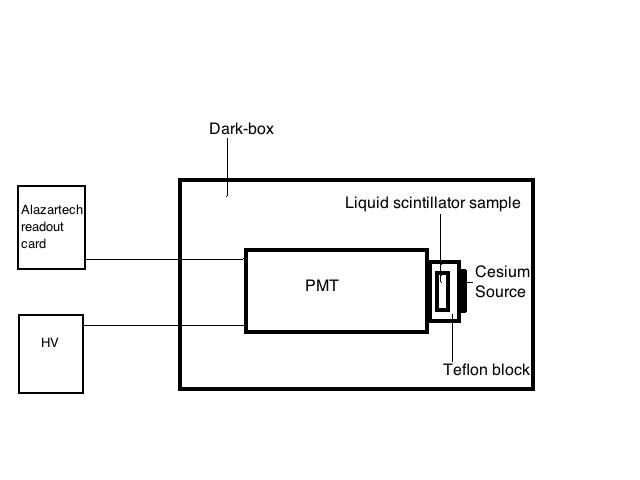
\includegraphics[scale=0.6]{graphs/Diagram_Darkbox.png}
\caption[]{Schematic view of the light yield measurement setup. \label{setup_fig}}
\end{center}
\end{figure}

\subsection{Absorption and Emission Setup}
\subsubsection{Setup}
A Perkin Elmer Lambda 25 UV/Vis is used for measuring the emission spectrum and a Shimadzu UV3101 for measuring absorption spectrum of the QD doped liquid scintillators. The instruments work via a double-beam setup. White light from deuterium UV lamp and a halogen lamp produce the beams. \cite{|}

\subsubsection{Sample Handling and Procedure}
To measure the absorption spectrum of each quantum-dot sample, the following procedure is executed. A (1~cm$\times$1~cm$\times$3.5~cm) UV-transparent quartz cell (Starna 21-Q-10 \cite{starnacells}) is rinsed with toluene to dissolve any residue on the wall. Next, the cell is soaked in hydrochloric acid for 5 minutes to clean the cell and destroy any remaining QD. To wash away the hydrochloric acid and the residue QD constituents, the quartz cell is rinsed with distilled water and is then subjected to three iterations of liquid isopropyl alcohol evaporated by nitrogen gas. Since all of the QD samples are dissolved in toluene, a background absorption spectrum analysis is required to isolate the quantum-dot spectrum.  The cell is filled wplaced into the Shimadzu UV3101, and a background scan is performed. Next, the toluene is removed from the cell and replaced by the QD sample of choice. Finally, The sample is inserted back into the spectrophotometer, and a scan is initiated. % This is repeated for each QD candidate listed in \ref{quantum_dots_table}.

The cleaning procedure for the emission spectrum measurements is the same as the procedure for the absorption trials. The emission spectrum is measured by a Perkin Elmer Lambda 25 UV/Vis and does not require a background toluene scan. 

\section{Results}
\label{analysis_results_sec}
This section presents the analysis methodology as well as the main results, namely the light yield measurements as a function of PPO concentrations for each of the solvents listed in Table \ref{solvents_table} and for the different QDs listed in Table \ref{quantum_dots_table} dissolved in toluene with 2~g/L of PPO added. The emission and absorption spectrum of the QD scintillators are also measured.
 
\subsection{Light Yield}\label{ly_analysis_sec}
\begin{figure}[tbh]
        \begin{center}
        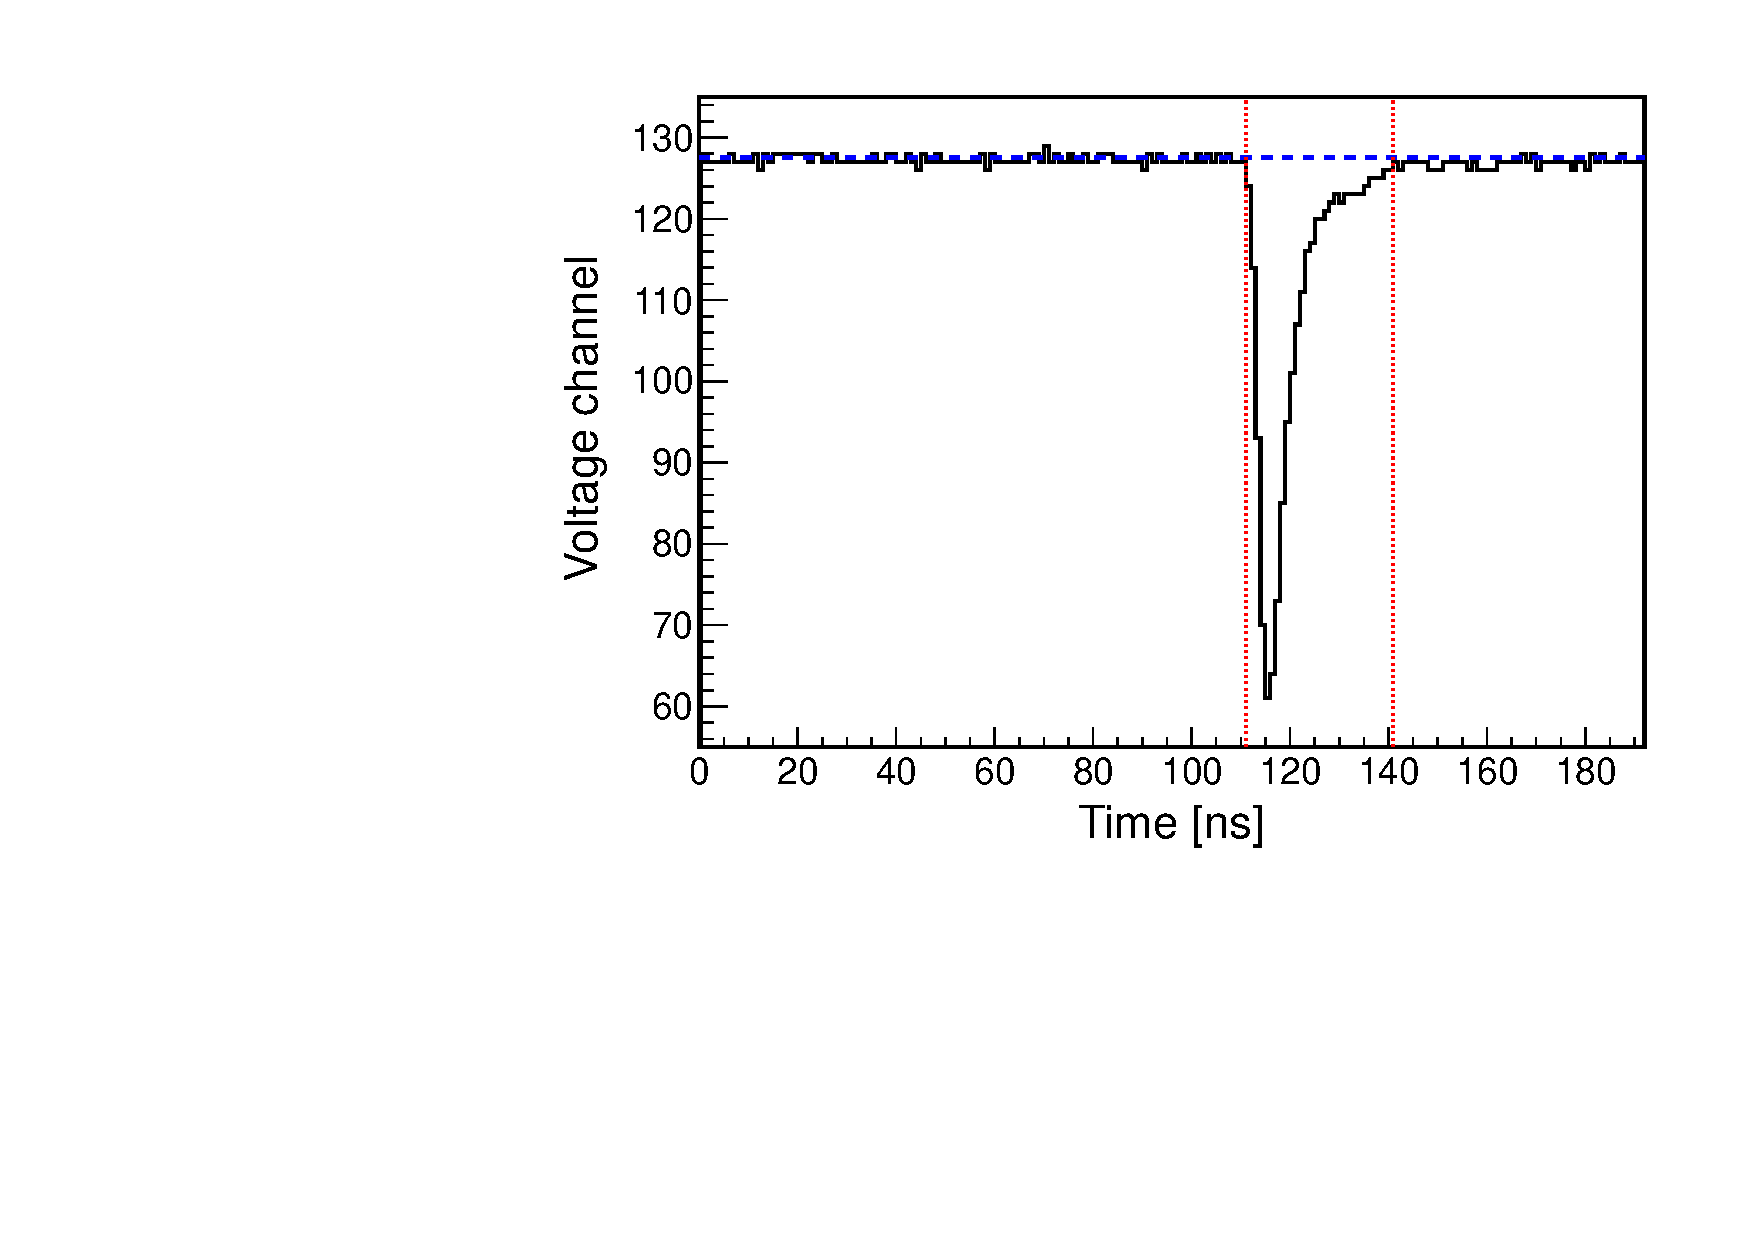
\includegraphics[scale=0.6] {graphs/14August2013_toluene_5gL_PPO_processed_waveform_paper.pdf}
\caption[]{Example waveform recorded by the AlazarTech digitizer card. For each waveform, 192 samples are taken with a rate of 1Gs/s. The blue, dashed line is the baseline which is calculated for each waveform. The red, dotted lines show the start and stop time for the main pulse in this waveform. Integration of the baseline subtracted waveform between start and stop yields 520. The trigger threshold is set at voltage channel 116. \label{waveform_fig}}
\end{center}
\end{figure}

\subsubsection{Signal Analysis}
%An example single waveform is shown in Figure \ref{waveform_fig}. Each waveform consists of 512 voltage samples. At a rate of 1~Gs/s one waveform thus spans 512~ns. The voltage range is [2~V,-2~V] with a resolution of 8-bit, 256 channels. The sampling is therefore done with voltage channels of size $\approx$ 0.0156~V. The amount of light collected is proportional to the the charge of a given pulse. Thus, the integral over the voltage pulse has to be calculated. To do this, the following steps are carried out for each waveform: 
\begin{itemize}
\item Baseline: At the beginning of each waveform, 100 samples are averaged to get the baseline value. 
\item Pulse finder: Pulses are defined as a consecutive series of samples below the rounded baseline value.
\item Pulse times: For each pulse the start time is defined as the time where the waveform falls below the rounded baseline value. The stop time is set once the pulse reaches this value again.  
\item Charge: The integral of the baseline-subtracted waveform between the start and stop times.  
\end{itemize}

The duration of each run is around thirty minutes and during this time on the order of $3\cdot10^5$ waveforms are recorded. Each pulse corresponds to one gamma ray interacation within the liquid scintillator sample. The amount of light collected by the PMT is dependent on the scattering angle of the electron that is produced by Compton scattering of the 0.662 MeV gamma ray. The result of the charge calculation is placed in a histogram, Figure \ref{ChargeSpec_fig}. Since the Compton effect is the dominant mechanism, this histogram is a Compton spectrum. The events where the Compton scattered electron obtained close to the maximal energy, 478~keV for the 662~keV gammas from $^{137}$Cs, is associated with events at the right end of this spectrum. %Since we are interested in the largest pulses close to the Compton edge we can simply use the charges of all the pulses.
Multiple pulses are found for each waveform, including baseline fluctuations. The small fake pulses from baseline fluctuations did not affect analysis. In order to compare different scintillator mixtures, the charge where the number of events dropped to half of the Compton edge maximum is compared, Figure \ref{ChargeSpec_fig}. This quantity is proportional to the scintillator light yield. For practical reasons and because this study only looks at relative light yield, results are presented in arbitrary charge units instead of real charge units.


\subsubsection{Investigation of Uncertainties}
This section focuses on the reproducibility of a measurement and estimates the error of a single measurement based on the sample handle procedure defined in Section \ref{ly_setup_sec}. 

The error due to differences in the procedure of coupling the scintillator cell to the PMT glass is measured. For this test, the same sample, LAB with 5~g/L PPO, is sealed in the cell and only the coupling is renewed. The RMS divided by the sample mean for several trials is 0.30~\%. This number is used as a rough estimate for the relative error of a single measurement due to differences in the coupling. The small uncertainty in the determination of the charge value from the histograms, Figure \ref{ChargeSpec_fig}, is already included here. The relative spread of 0.30~\% is negligible compared to other uncertainties discussed below.   

The effect of oxygen is also studied quantitatively. A comparatively 24-day old sample of DIN HP with 5~g/L PPO is purged with nitrogen bubbles for 10 minutes as in the standard measurement procedure and is measured. Then the sample is opened and left in contact with oxygen for 15 minutes. It is then re-measured without nitrogen purging. The charge value dropped by 2.04~\%. After an additional ~3 hours of contact with oxygen the same is measured. The relative difference between the first and the last measurement is about 6.92~\%, indicating the importance of nitrogen purging and reproducible procedures in preventing oxygen from entering the scintillator. 

In order to estimate the total error of a single light yield measurement, the same sample with the full sample change protocol, as described in Section \ref{ly_setup_sec}, is measured repeatedly. For these measurements an older sample, 7 weeks after mixing, of DIN HP is used as well as a standard DIN sample, 3-4 weeks old. For the older samples, 10 minutes of nitrogen purging is not sufficient to remove oxygen. The effect of differences in the oxygen removal is included in these reproducibility measurements. However, it is difficult to assess exactly how oxygen contamination affects the measurements when the full measurement protocol is applied. The RMS for these data sets 
is is about 3.70~\% and is regarded as a rough estimate of the relative uncertainty of a single light yield measurement.

\begin{figure}[tbh]
        \begin{center}
        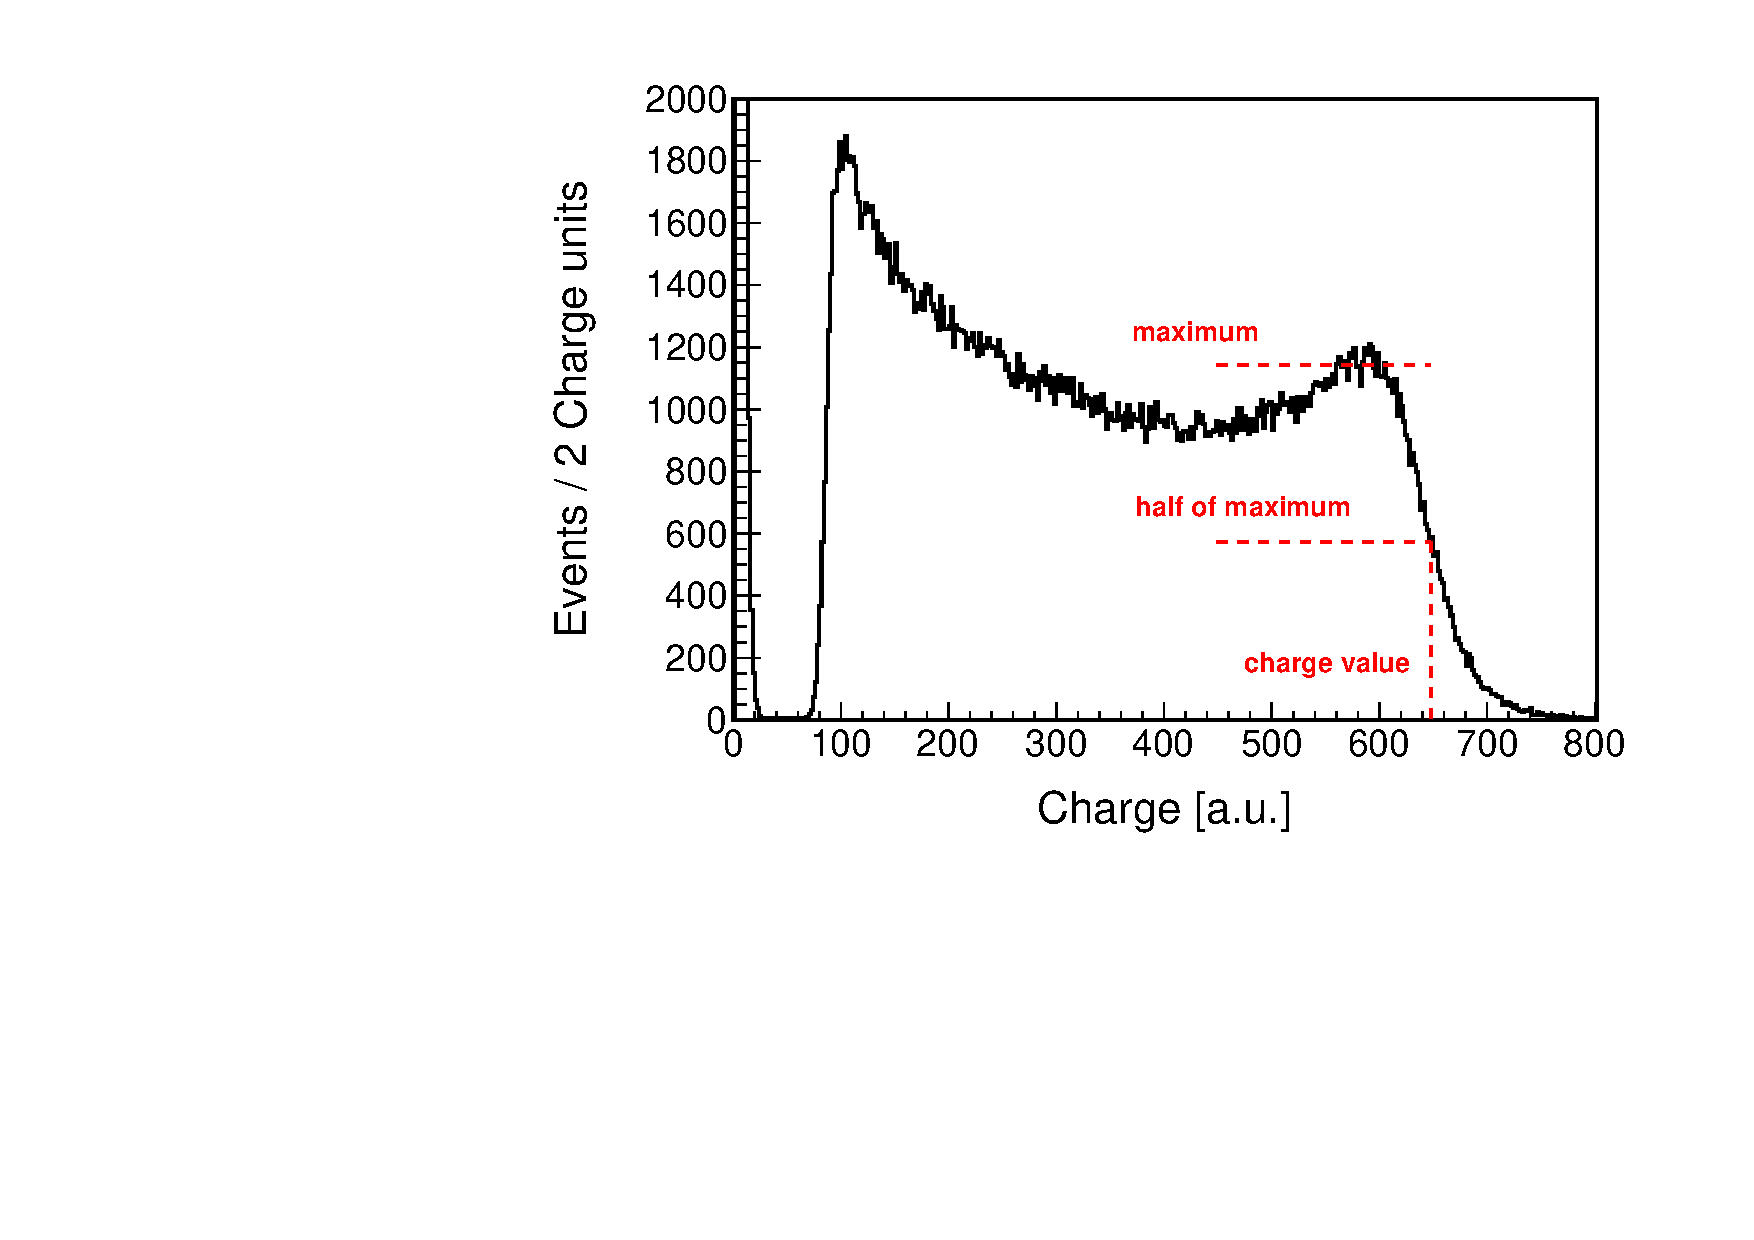
\includegraphics[scale=0.6]{graphs/toluene_5gL_PPO_Floats_final.pdf}
\caption[]{Example charge spectrum. To compare different scintillators, the charge at a characteristic point close to the true Compton edge is determined. \label{ChargeSpec_fig}}
 \end{center}
\end{figure}

\subsubsection{Light Yield Results}\label{ly_results}
Table \ref{fitresult_table} contains the light yield results for the different liquid scintillator candidates described in Table \ref{solvents_table}.

In Figure \ref{fitresult_table}, each plot shows the solvent's characteristic charge at the Compton edge as a function of PPO concentration in g/L. Concentrations of 0.5 g/L, 1 g/L, 2 g/L, 5 g/L, 10 g/L and 50 g/L have been used. Tables \ref{ChargeResults_fig} and \ref{Toluene_ChargeResults_fig} include the fit results; the parameters p1, p2 and p3 describe the light yield normalization,
the energy transfer from solvent to solute and the self-quenching effect, respectively.

As clearly stated in Table \ref{Toluene_ChargeResults_fig}, toluene produces the highest light yield around 2.2~g/L.  QD scintillators are doped with 2~g/L PPO for comparison with 2~g/L PPO in toluene. The light yield as a function of QD emission wavelength is plotted in Figure \ref{ly_QD}.

\begin{table}
\caption{Listed below are the fit results for each solvent's data set. The fit parameters and their errors are given and their respective $\chi^{2}$ values, and the probabilities to get a worse $\chi^{2}$ than the observed one. Since we have 6 data points and 3 parameters in the fit the number of degrees of freedom is 3. \label{fitresult_table}}

  \begin{center}
    \begin{tabular}{lllllll}
       Solvent & $p_1$ [a.u.] & $p_2$ [g/L] & $p_3$ [g/L] & $\chi^{2}$ & prob. \% & max. LY\\
       \hline\hline\\[-5px]
       Toluene  & $681 \pm 10$  & $0.09 \pm 0.014$  & $0.019 \pm 0.001$ & 0.55 & 91 & 627 (at 2.2~g/L)\\
       PC & 578 $\pm$ 47  & 2.09 $\pm$ 0.37  & 0.014 $\pm$ 0.004  & 5.30  & 15  & 422 (at 12.2~g/L)\\
       LAB & 525 $\pm$ 24  & 0.36 $\pm$ 0.01  & 0.013 $\pm$ 0.003  & 4.33  & 23 & 462 (at 5.3~g/L)\\
       PXE & 694 $\pm$ 25  & 0.48 $\pm$ 0.96  & 0.013 $\pm$ 0.002 & 2.55  & 47 & 596 (at 6.1~g/L) \\
       DIN & 668 $\pm$ 19  & 0.27 $\pm$ 0.01  & 0.007 $\pm$ 0.001  & 2.34  & 50 & 613 (at 6.2~g/L)  \\
       DIN HP & 673 $\pm$ 40 & 0.19 $\pm$ 0.08 & 0.005 $\pm$ 0.003  & 10.6  & 1 & 631 (at 6.1~g/L) \\
       PCH & 634 $\pm$ 29  & 0.34 $\pm$ 0.07  & 0.012 $\pm$ 0.003 & 6.11  & 11 & 562 (at 5.4 ~g/L) \\
      \hline \hline
    \end{tabular}
  \end{center}
\end{table}

\begin{figure}[tbh]
        \begin{center}
        \subfigure[PC]{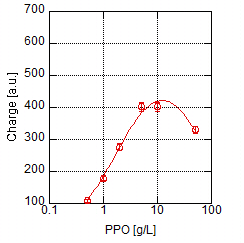
\includegraphics[scale=0.30]{graphs/Light_Yield/PC_Light_Yield.png}}
        \subfigure[LAB]{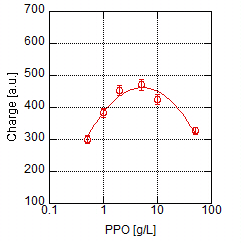
\includegraphics[scale=0.30]{graphs/Light_Yield/LAB_Light_Yield.png}}
        \subfigure[PXE]{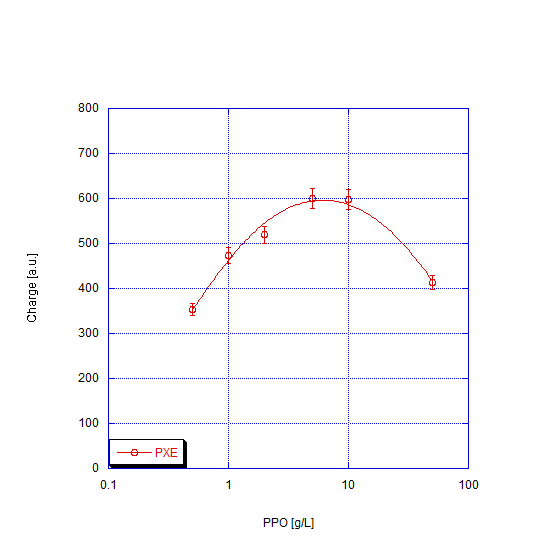
\includegraphics[scale=0.30]{graphs/Light_Yield/PXE_Light_Yield.png}}
        \subfigure[DIN]{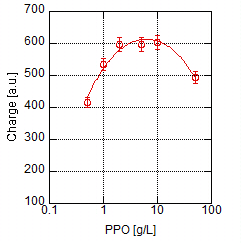
\includegraphics[scale=0.30]{graphs/Light_Yield/DIN_Light_Yield.png}}
        \subfigure[DIN HP]{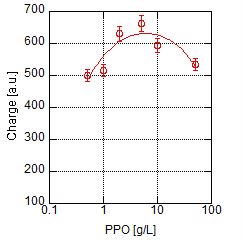
\includegraphics[scale=0.30]{graphs/Light_Yield/DIN_HP_Light_Yield.png}}
        \subfigure[PCH]{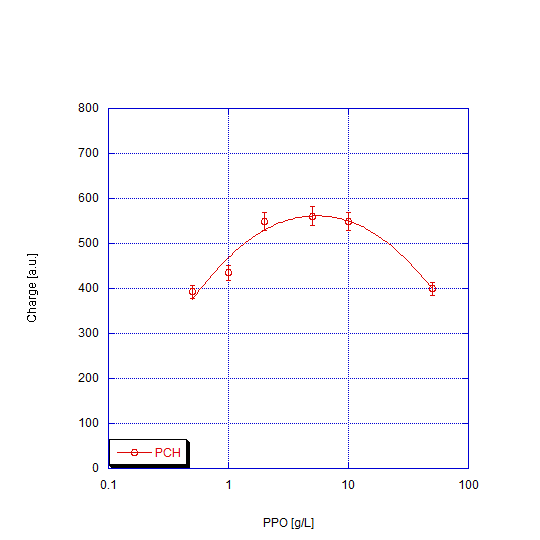
\includegraphics[scale=0.30]{graphs/Light_Yield/PCH_Light_Yield.png}}
\caption[]{Show the charge value at the Compton edge (proportional to the light yield) for each of the 6 concentrations of PPO for six of the liquid scintillator candidates. A relative error of $3.7~\%$ was used for each measurement. The red lines show the fit of equation \ref{fit_eq}. Note that the x-axis is logarithmic; the PPO concentrations span two orders of magnitude. %The rise of the LY at low concentrations is faster than the drop due to self-quenching at high concentrations.
  \label{ChargeResults_fig}}
        \end{center}
\end{figure}

\begin{figure}[tbh]
        \begin{center}
        \subfigure[Toluene]{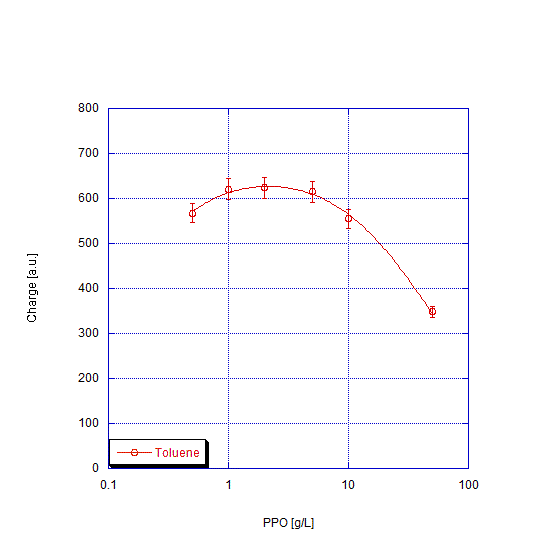
\includegraphics[scale=0.30]{graphs/Light_Yield/Toluene2014_Light_Yield.png}}
\caption[]{Show the charge value at the Compton edge (proportional to the light yield) for each of the 6 concentrations of PPO for toluene. A relative error of $3.7~\%$ was used for each measurement. The red lines show the fit of equation \ref{fit_eq}. Note that the x-axis is logarithmic; the PPO concentrations span two orders of magnitude. %The rise of the LY at low concentrations is faster than the drop due to self-quenching at high concentrations.
  \label{Toluene_ChargeResults_fig}}
        \end{center}
\end{figure}




\begin{figure}[tbh]
        \begin{center}
        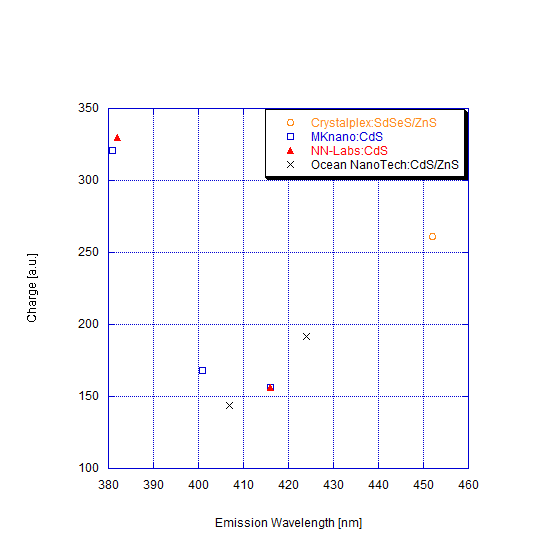
\includegraphics[scale=0.3] {graphs/Light_Yield/QDots_Light_Yield.png}
\caption[]{The light yield of quantum-dot doped toluene scintillators with 2~g/L of PPO versus emission wavelength of the QDs.\label{ly_QD}}
\end{center}
\end{figure}

\subsection{Emission and Aborption Spectrum of Quantum-Dot Doped Liquid Scintillators}

\subsubsection{Signal Analysis}
Various trials are conducted to test the output signal of both the Perkin Elmer Lambda 25 UV/Vis and the Shimadzu UV3101 spectrophotometers\cite{lindley13}. The error is described by the following equation:
 \ref{Absorption_equ}.

\begin{equation}
\label{Absorption_equ}
A(x)=\log_{10}\Big(\frac{I(x)}{I(0)}\Big)
\end{equation}
where  $I(0)$ is the intensity of the beam before transiting the quartz cell and $I(x)$ is the intensity after it passes through the cell. 

The errors for the Perkin and Shimadzu spectrophotometers are $A=\pm0.00075$ and $A=\pm0.002$ respectfully. These errors are in close agreement with the manufactures specifications\cite{?}.

\subsubsection{Absorption and Emission Results}\label{abs_emi_results}
The absorption and emission spectrum of the QDs were extensively probed, and the results are graphed in Figures \ref{abs_spec} and \ref{emi_spec} respectfully. As stated in Section \ref{qd_sec} and proved in \ref{ly_results}, the light yield of the QD doped scintillators is much lower than that of just toluene with PPO. This is due to the overlap in emission and absorption QD spectrum coupled with low quantum efficiency \cite{lindley14}. (I'm creating a figure that shows the overlap for emission and absorption for each quantum dot). The absorption spectrum of the QD doped liquid scintillators are clearly narrower than that of toluene doped with 2 g/L PPO.
(How can we back this? Need to take an absorption and emission scan of toluene + 2g/L PPO.)
%Discuss the shift of emission spectrum (Measure Toluene with PPO emission Spectrum)

\begin{figure}[tbh]
        \begin{center}
        \subfigure[NN-Labs]{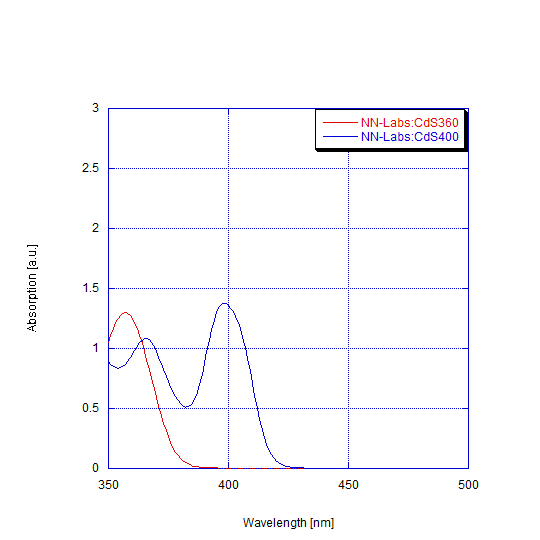
\includegraphics[scale=0.29]{graphs/Emission_Absorption/NN_Labs_Abs.png}}
        \subfigure[mkNano]{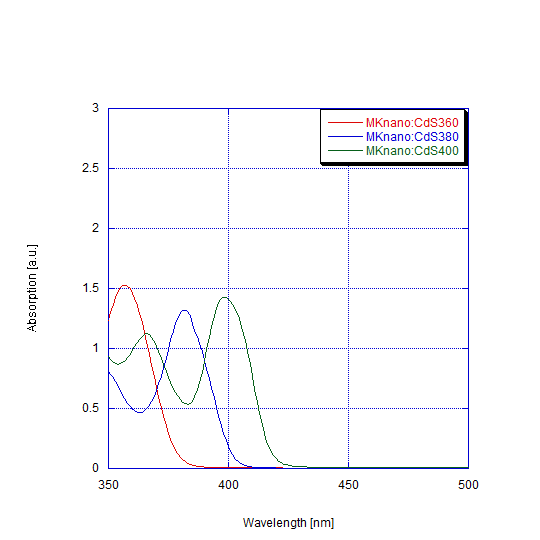
\includegraphics[scale=0.29]{graphs/Emission_Absorption/mkNano_Abs.png}}
        \subfigure[Ocean NanoTech]{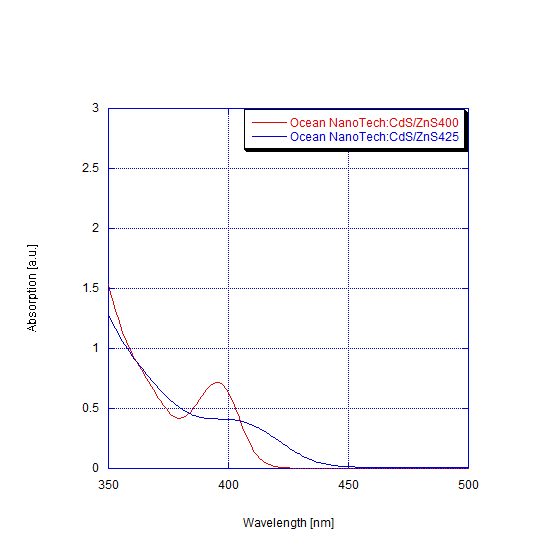
\includegraphics[scale=0.29]{graphs/Emission_Absorption/Ocean_NanoTech_Abs.png}}
        \subfigure[Crystalplex]{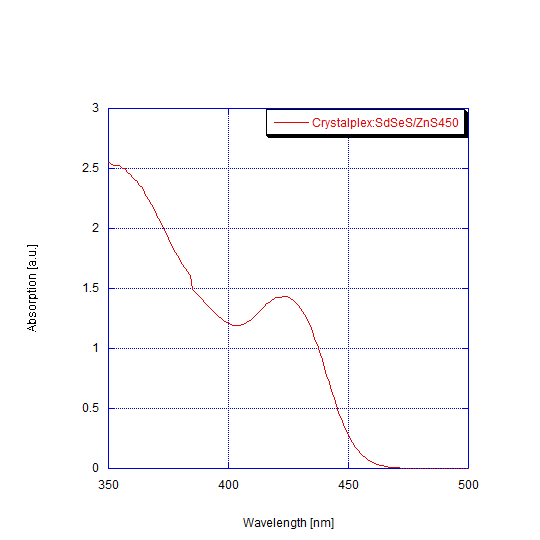
\includegraphics[scale=0.29]{graphs/Emission_Absorption/Crystalplex_Abs.png}}
\caption[]{Absorption spectrum of the quantum-dots listed in Table \ref{quantum_dots_table} dissolved in toluene and grouped by manufacturer.}\label{abs_spec}
\end{center}
\end{figure}

\begin{figure}[tbh] 
        \begin{center}
        \subfigure[]{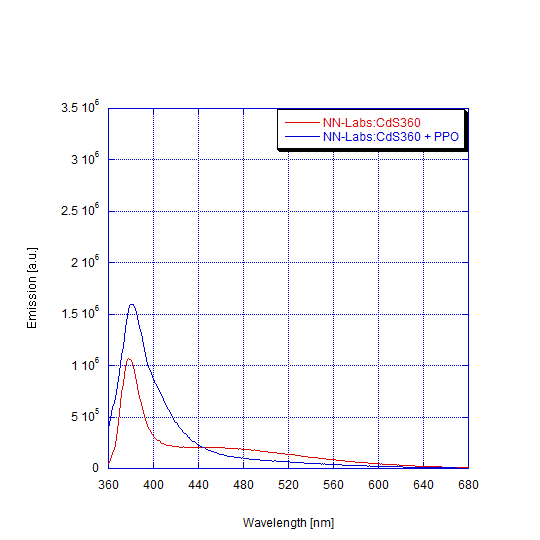
\includegraphics[scale=0.28]{graphs/Emission_Absorption/NNLabs_360nm_Emi.png}}
        \subfigure[]{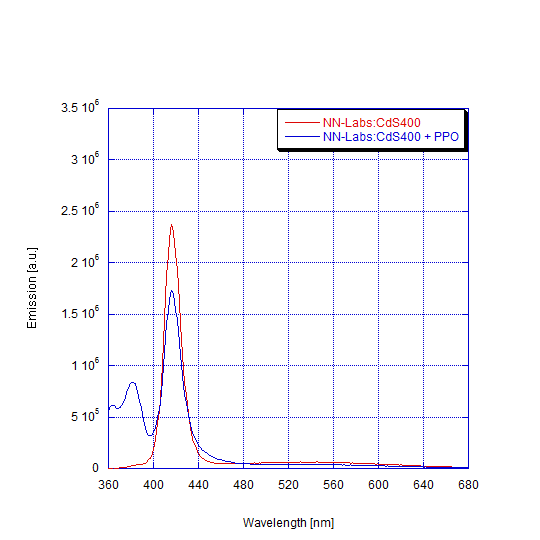
\includegraphics[scale=0.28]{graphs/Emission_Absorption/NNLabs_400nm_Emi.png}}
        \subfigure[]{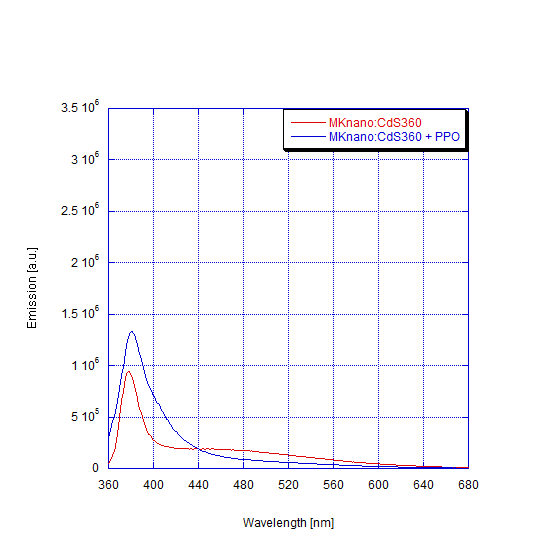
\includegraphics[scale=0.28]{graphs/Emission_Absorption/mkNano_360nm_Emi.png}}
        \subfigure[]{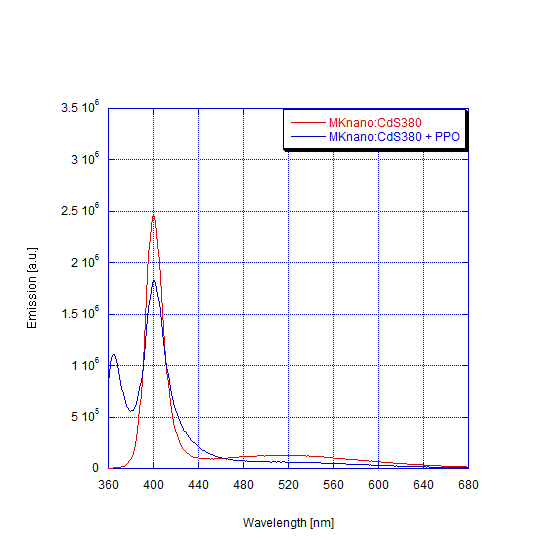
\includegraphics[scale=0.28]{graphs/Emission_Absorption/mkNano_380nm_Emi.png}}
        \subfigure[]{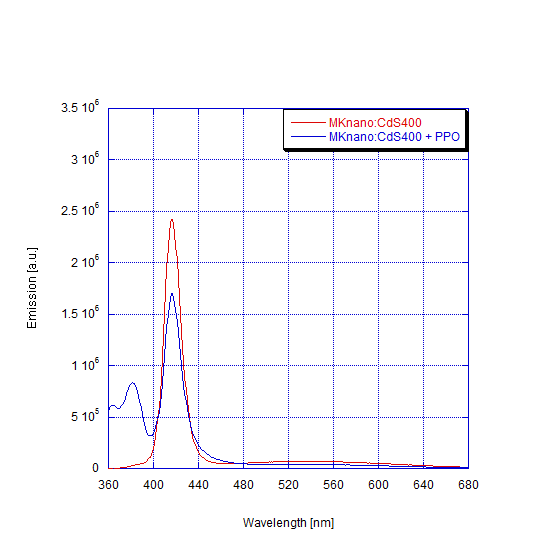
\includegraphics[scale=0.28]{graphs/Emission_Absorption/mkNano_400nm_Emi.png}}
        \subfigure[]{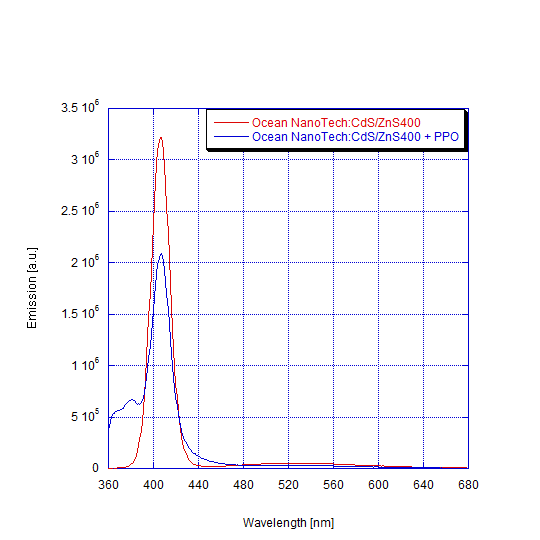
\includegraphics[scale=0.28]{graphs/Emission_Absorption/Ocean_NanoTech_400nm_Emi.png}}
        \subfigure[]{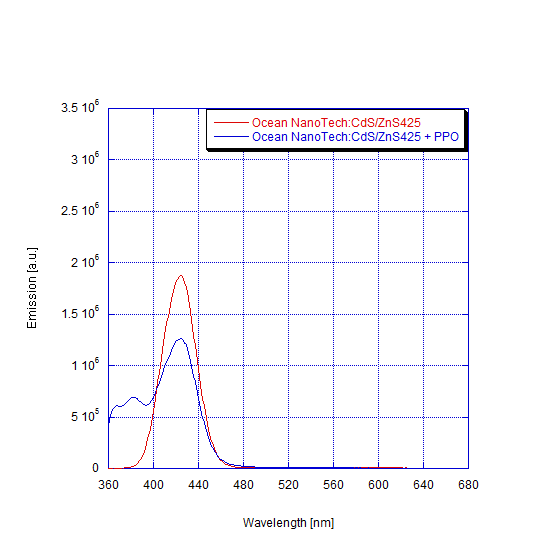
\includegraphics[scale=0.28]{graphs/Emission_Absorption/Ocean_NanoTech_425nm_Emi.png}}
        \subfigure[]{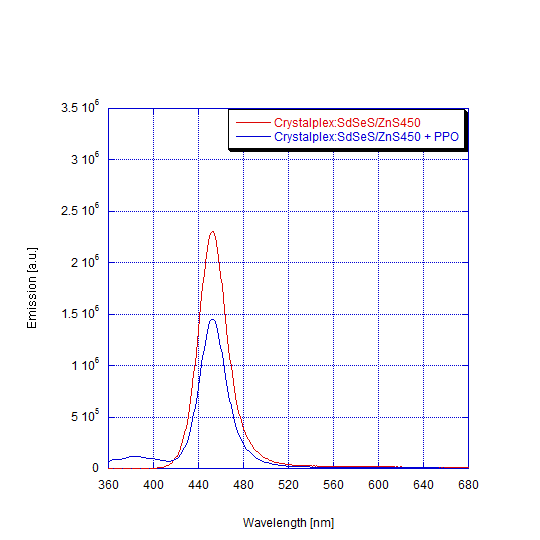
\includegraphics[scale=0.28]{graphs/Emission_Absorption/Crystalplex_Emi.png}}
\caption[]{Emission spectrum of the quantum-dots listed in Table \ref{quantum_dots_table} dissolved in toluene with and without 2~g/L of PPO added.\label{emi_spec}}
\end{center}
\end{figure}


\section{Conclusion}
Detection of low energy events in liquid scintillators require high light yield and preservation of Cherenkov radiation. This study  successfully measures and models the light yield of seven scintillator liquids as a function of wavelength-shifter concentration in order to find the maximum light yield of each candidate. Furthermore, an extensive study on the effects of quantum-dot doping of toluene with 2 g/L of PPO in solution are analyzed. QDs are able to reduce the width and tune the location of the absorption spectrum peak. This allows the quantum efficiency of the photocathode to be matched and minimized the amount of Cherenkov radiation absorbed by the liquid scintillator.

Regrettably,QDs significantly reduce the light yield of scintillators. With improved technology in quantum dot production, QDs with better characteristics such as shorter emission wavelengths are expected to become available in the near future. These QDs should be able to improve the light yield of quantum dot-doped scintillator. 


\begin{thebibliography}{35}
\bibitem{majorana37}
E.~Majorana, \emph{Teoria simmetrica dell'elettrone e del positrone}, \emph{Il Nuovo Cimento} {\bf 14} (1937) 171. 

\bibitem{furry39}
W.H.~Furry, \emph{On Transition Probabilities In Double Beta-Disintegration}, \emph{Phys. Rev.} {\bf 56} (1939) 1184. 

\bibitem{Zuber}
K.~Zuber, \emph{Neutrino Physics}, Taylor and Francis Group, 2004.

\bibitem{tabledb95}
V.I.~Tretyak, Y.G.~Zdesenko, \emph{Tables of double beta decay data}, \emph{Atomic Data and Nuclear Data Tables} {\bf 61} (1995) 43. 

\bibitem{elliott02}
S.R.~Elliott and P.~Vogel, \emph{Double Beta Decay}, \href{http://www.annualreviews.org/doi/abs/10.1146/annurev.nucl.52.050102.090641}{\emph{Annu. Rev. Nucl. Part. S.} {\bf 52} (2002) 115}.

\bibitem{barabash11}
A.~Barabash, \emph{Double beta decay experiments}, Phys. Part. Nucl. {\bf 42} (2011) 613 [\href{http://arxiv.org/abs/1107.5663}{arXiv:1107.5663}].

\bibitem{schwingenheuer13}
B.~Schwingenheuer, \emph{Status and prospects of searches for neutrinoless double beta decay}, \emph{Ann. Phys.} {\bf 525} (2013) 269.

\bibitem{cremonesi13}
O.~Cremonesi and M.~Pavan, \emph{Challenges in Double Beta Decay}, \href{http://arxiv.org/abs/1310.4692}{arXiv:1310.4692}.

\bibitem{schechter82}
J.~Schechter and J.W.F.~Valle, \emph{Neutrinoless double-$\beta$ decay in SU(2)$\times$U(1) theories}, \emph{Phys. Rev. D} {\bf 25} (1982) 2951.  

\bibitem{klapdor04}
H.V.~Klapdor-Kleingrothaus, I.V.~Krivosheina, A.~Dietz and O.~Chkvorets, \emph{Search for neutrinoless double beta decay with enriched 76Ge in Gran Sasso 1990-2003}, \emph{Phys. Lett. B} {\bf 586} (2004) 198.

\bibitem{klapdor06}
H.V.~Klapdor-Kleingrothaus and I.~Krivosheina, \emph{The evidence for the observation of 0$\nu\beta\beta$ decay: the identification of 0$\nu\beta\beta$ events from the full spectra}, \emph{Mod. Phys. Lett. A} {\bf 21} (2006) 1547 (2006).

\bibitem{heidelbergmoscow01}
H.V.~Klapdor-Kleingrothaus et al. (Heidelberg-Moscow Collaboration), \emph{Latest results from the HEIDELBERG-MOSCOW double beta decay experiment}, \emph{Eur. Phys. J. A} {\bf 12} (2001) 147.

\bibitem{gerda13}
M.~Agostini et al. (GERDA collaboration), \emph{Results on Neutrinoless Double-$\beta$ Decay of $^{76}$Ge from Phase I of the GERDA Experiment}, \emph{Phys. Rev. Lett.} {\bf 111} (2013) 122503. 

\bibitem{kamlandzen13}
A.~Gando et al. (KamLAND-Zen Collaboration), \emph{Limit on Neutrinoless $\beta\beta$ Decay of $^{136}$Xe from the First Phase of KamLAND-Zen and Comparison with the Positive Claim in $^{76}$Ge}, \emph{Phys. Rev. Lett.} {\bf 110} (2013) 062502.

\bibitem{snoplus10}
C.~Kraus, S.J.M.~Peeters, \emph{The rich neutrino programme of the SNO+ experiment}, \emph{Prog. Part. Nucl. Phys.} {\bf 64} (2010) 273.

\bibitem{hartnell12}
J.~Hartnell for the SNO+ collaboration, \emph{Neutrinoless Double Beta Decay with SNO+}, \emph{J. Phys. Conf. Ser.} {\bf 375} (2012) 042015.

\bibitem{birks64}
J.B.~Birks, \emph{The Theory and Practice of Scintillation Counting}, Pergamon Press, 1964.

\bibitem{lindley14}
C.~Aberle, J.J.~Li, S.~Weiss and L.~Winslow, \emph{Measuring directionality in double-beta decay and neutrino interactions with kiloton-scale scintillation detectors }, \jinst{9}{2014}{P06012}.

\bibitem{lindley13}
C.~Aberle, J.J.~Li, S.~Weiss and L.~Winslow, \emph{Optical properties of quantum-dot-doped liquid scintillators}, \jinst{8}{2013}{P10015}.

\bibitem{sigmaaldrich}
http://www.sigmaaldrich.com (2014).

\bibitem{cepsa}
http://www.cepsa.com (2014). 

\bibitem{dixiechemical}
http://www.dixiechemical.com (2014).

\bibitem{perkinelmer}
http://www.perkinelmer.com (2014).

\bibitem{nnLabs}
http://www.nn-labs.com (2014).

\bibitem{mkNano}
http://mknano.com (2014).

 \bibitem{oceanNanotech}
 http://www.oceannanotech.com (2014).
 
 \bibitem{crystalplex}
 http://www.crystalplex.com (2014).

\bibitem{starnacells}
http://www.starnacells.com (2014).  

\bibitem{foerster48}
T.~F\"orster, \emph{Zwischenmolekulare Energiewanderung und Fluoreszenz}, \emph{Ann. Phys.} {\bf 2} (1948) 55.

\bibitem{foerster59}
T.~F\"orster, \emph{Transfer Mechanisms of electronic excitation}, \emph{Discuss. Faraday Soc.} {\bf 27} (1959) 7.

\bibitem{dexter53}
D.L.~Dexter, \emph{A theory of sensitized luminescence in solids}, \emph{J. Chem. Phys.} {\bf 21} (1953) 836.

\bibitem{buck07}
C.~Buck, F.X.~Hartmann, D.~Motta, S.~Sch\"onert, \emph{Energy transfer and light yield properties of a new highly loaded indium(III) $\beta$-diketonate organic scintillator system}, \emph{Chem. Phys. Lett.} {\bf 435} (2007) 252. 

\bibitem{aberle11}
C.~Aberle, C.~Buck, F.X.~Hartmann and S.~Sch\"onert, \emph{Light yield and energy transfer in a new Gd-loaded liquid scintillator}, \emph{Chem. Phys. Lett.} {\bf 516} (2011) 257.  


\bibitem{hamamatsupmt}
Hamamatsu Photonics K.K., \emph{Photomultiplier Tubes R1828-01, R2059} (data sheet), accessed March, 2014: http://www.hamamatsu.com/resources/pdf/etd/R1828-01\_R2059\_TPMH1259E04.pdf.

\bibitem{hamamatsubase}
Hamamatsu Photonics K.K., \emph{D-Type Socket Assemblies} (data sheet), accessed March, 2014: http://www.hamamatsu.com/resources/pdf/etd/PMT\_92-103\_e.pdf.

\bibitem{alazartech}
http://www.alazartech.com (2014).

\end{thebibliography}
\end{document}

%Charge figure 2 and 3, and table 3 with Chi-Square Fit
%Should the section on oxygen's afffect on LY be included
%Should the numbers in the uncertainties be changed?